\documentclass[border=10pt]{standalone}
\usepackage{xcolor}
\definecolor{slidebg}{HTML}{f0f1eb}
\pagecolor{slidebg}
\usepackage{tikz}
\usepackage{amsmath}
\usetikzlibrary{arrows.meta, shapes.geometric, positioning}

\definecolor{gruvblue}{HTML}{458588}
\definecolor{gruvpurple}{HTML}{b16286}
\definecolor{gruvgray}{HTML}{928374}

\begin{document}
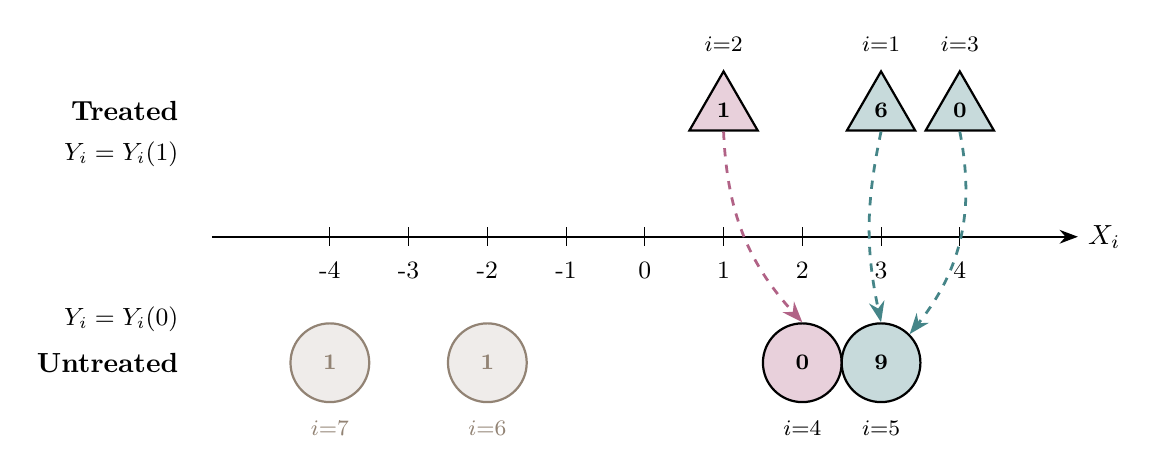
\begin{tikzpicture}[
  >=Stealth,
  tnode/.style={regular polygon, regular polygon sides=3,
    minimum size=10mm, draw=black, line width=0.8pt, inner sep=0pt,
    font=\footnotesize\bfseries},
  cnode/.style={circle, minimum size=10mm, draw=black, line width=0.8pt,
    inner sep=0pt, font=\footnotesize\bfseries},
  yval/.style={font=\footnotesize},
  arr/.style={->, dashed, line width=1pt}
]

% ---- Number line ----
\draw[->, black, line width=0.8pt] (-5.5,0) -- (5.5,0) node[right, font=\normalsize\itshape] {$X_i$};
\foreach \x in {-4,-3,...,4} {
  \draw[black] (\x,0.12) -- (\x,-0.12);
  \node[below, font=\small, black] at (\x,-0.2) {\x};
}

% ---- Group labels ----
\node[font=\normalsize\bfseries, anchor=east] at (-5.8,1.6) {Treated};
\node[font=\small, anchor=east] at (-5.8,1.05) {$Y_i = Y_i(1)$};
\node[font=\normalsize\bfseries, anchor=east] at (-5.8,-1.6) {Untreated};
\node[font=\small, anchor=east] at (-5.8,-1.05) {$Y_i = Y_i(0)$};

% ---- Treated units (Y inside shape, i as label) ----
\node[tnode, fill=gruvpurple!30] (t2) at (1,1.6) {1};
\node[yval, above=1mm of t2] {$i{=}2$};

\node[tnode, fill=gruvblue!30] (t1) at (3,1.6) {6};
\node[yval, above=1mm of t1] {$i{=}1$};

\node[tnode, fill=gruvblue!30] (t3) at (4,1.6) {0};
\node[yval, above=1mm of t3] {$i{=}3$};

% ---- Matched controls ----
\node[cnode, fill=gruvpurple!30] (c4) at (2,-1.6) {0};
\node[yval, below=1mm of c4] {$i{=}4$};

\node[cnode, fill=gruvblue!30] (c5) at (3,-1.6) {9};
\node[yval, below=1mm of c5] {$i{=}5$};

% ---- Unmatched controls ----
\node[cnode, fill=gruvgray!15, draw=gruvgray, text=gruvgray] (c6) at (-2,-1.6) {1};
\node[yval, below=1mm of c6, text=gruvgray] {$i{=}6$};

\node[cnode, fill=gruvgray!15, draw=gruvgray, text=gruvgray] (c7) at (-4,-1.6) {1};
\node[yval, below=1mm of c7, text=gruvgray] {$i{=}7$};

% ---- Match arrows ----
% i=1 (X=3) → i=5 (X=3)
\draw[arr, gruvblue] (t1.south) to[bend right=12] (c5.north);
% i=2 (X=1) → i=4 (X=2)
\draw[arr, gruvpurple] (t2.south) to[bend right=20] (c4.north);
% i=3 (X=4) → i=5 (X=3)
\draw[arr, gruvblue] (t3.south) to[bend left=25] (c5.north east);

\end{tikzpicture}
\end{document}
